\documentclass[12pt]{amsart}
\usepackage[margin=3cm]{geometry}                % See geometry.pdf to learn the layout options. There are lots.
\geometry{letterpaper}                   % ... or a4paper or a5paper or ... 
%\geometry{landscape}                % Activate for for rotated page geometry
%\usepackage[parfill]{parskip}    % Activate to begin paragraphs with an empty line rather than an indent
\usepackage{graphicx}
\usepackage{amssymb}
\usepackage{epstopdf}
\usepackage{siunitx}
\DeclareGraphicsRule{.tif}{png}{.png}{`convert #1 `dirname #1`/`basename #1 .tif`.png}
\title{\bigskip \bigskip   \vspace{50mm} Coupled Pendulums}
     
%%%%%%%%%%%%%%%\title{Coupled Pendulums \\ Intermediate Experimental Physics I} % Title

\author{Caspar \textsc{Lant}} % Author name

\date{\today} % Date for the report

\begin{document}

\bigskip
\maketitle % Insert the title, author and date
\begin{center}
Intermediate Experimental Physics I\\
\vfill
\begin{tabular}{l r}

Section: & 002\\
\\
Date Performed: & November 6, 2015 \\ % Date the experiment was performed
Date Due: & November 13, 2015\\
\\
Partners: & Sam Meier \\ % Partner names
Professor: & Prof. Andrew Kent\\ 
Instructor: & David Mykytyn % Instructor/supervisor
\end{tabular}
\end{center}
\vspace{50mm}
	
\pagebreak
\textbf{The Objective} of this week's experiment is to explore the interactions of two pendulums which share a common axis, as a way to frame our studies of waves and harmonic motion.\\\\
\textbf{Theoretical Background/Abstract: }
\paragraph{Way back in the mid 17th century, the brilliant Huygens noticed that the two grandfather clocks on his mantlepiece (who keeps two grandfather clocks on their mantlepiece?)  had fallen into synchrony! The pendulums that drove the two clocks were not oscillating in phase, as one might expect, but 180� out of phase. We will learn later that this is one of 2 normal modes that exist for a two-pendulum oscillating system. From here, Huygens formulated an equation that could generalize the motion of two pendulums. Before this, let's assume the following conditions, which give rise to force equations for each pendulum}
\paragraph{\\Let's assume that $l$ and $m$ are the same for each pendulum, that each pendulum oscillates in the same plane, angles are small;  $ sin\theta \approx \theta, $ and that $F_a = - Kl(\theta_a- \theta_b), $ $F_b = - Kl(\theta_a- \theta_b)$, $\Sigma F = 0$}

\begin{equation}
ml \frac{d^2\theta_a}{dt^2} = -mg\theta_a - Kl_0 (\theta_a- \theta_b)
\end{equation}
\begin{equation}
\frac{d^2\theta_a}{dt^2}  + \frac{g}{l}\theta_a + K \frac{l_0}{ml} (\theta_a- \theta_b) = 0 ?
\end{equation}
\begin{equation}
\frac{d^2\theta_a}{dt^2}  + \omega^2 \theta_a + C (\theta_a- \theta_b) = 0 \\
\Big(\omega_0 = \sqrt{\frac{g}{l}}\Big)
\end{equation}
\paragraph{Where $l_0$ is the position of the spring coupling between the pendulums, with $l_0 = 0$ at the axis of oscillation}
\paragraph{\\Normal modes denote starting conditions under which the motion of the pendulum is stable, and constant in phase-space. This is to say that, if you start a two pendulum in one of its two normal modes, it will continue to oscillate in this mode, with no energy trade-off between the pendulums. These modes are eigenvectors of the equation to follow. The so-called ``slow mode'' is given by the initial condition $\theta_a = \theta_b$, and is shown in vector-form by $[1,1]$. The second, ``fast mode'' is given by $\theta_a = -\theta_b$, or $[1,-1]$}

\paragraph{\\For arrangements of pendulums that cannot be classified as either of the the system's two normal modes, we find the following equation:\\}

\begin{equation}
\vec{X}(t) = \left[\begin{array}{c}1 \\1\end{array}\right](a_{1}cos\omega_{1}t+ b_{1}sin\omega_{1}t) + 
\left[\begin{array}{c}1 \\-1\end{array}\right](a_{2}cos\omega_{2}t+ b_{2}sin\omega_{2}t)
\end{equation}

\newpage
\begin{figure}[ht!]
\centering
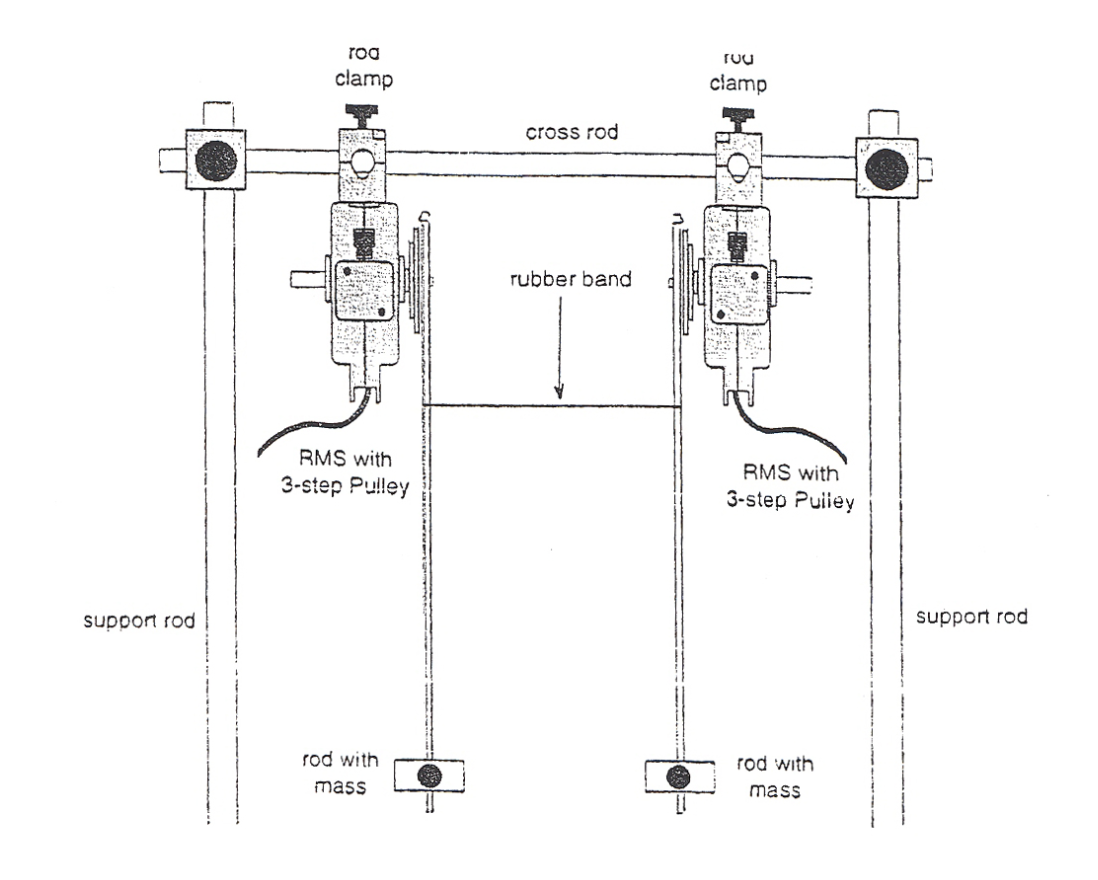
\includegraphics[width=100mm]{Figure.png}
\caption{Experimental Setup}
\end{figure}
\medspace
\textbf{Experimental Procedure}?
\smallskip
\begin{itemize}
\item Set up the two pendulum system in the manner detailed by the above diagram.
\item Connect the two rotary distance sensors to Data Studio via the provided interface.
\item Create a display in Data Studio that graphs the position of each distance sensor over time.
\item Match the frequency of one pendulum to that of its partner by adjusting the position of its mass. It's of note here that we disregard the mass of the rod in our calculations. 
\item Plot the oscillation of each pendulum in Data Studio and compute its frequency with a best-fit sine function.
\item Connect the rubber band to each pendulum at a distance of 5cm.
\item Start the pendulums off in the ``slow mode'' and record their oscillations in Data Studio. 
\item Do the same for the ``fast mode''.
\item Now for something more interesting: start the pendulum off in a ``non-normal'' mode by displacing one pendulum and keeping the other at zero position. Ensure the the angle of displacement is sufficiently small, in accordance with the paraxial approximation on page one.
\item Repeat each experiment for rubber band length distances 10cm, 15cm, 20cm, and so on. How does the position of the rubber band affect the rate of the pendulums' oscillation?
\end{itemize}

\begin{figure}[ht!]
\centering
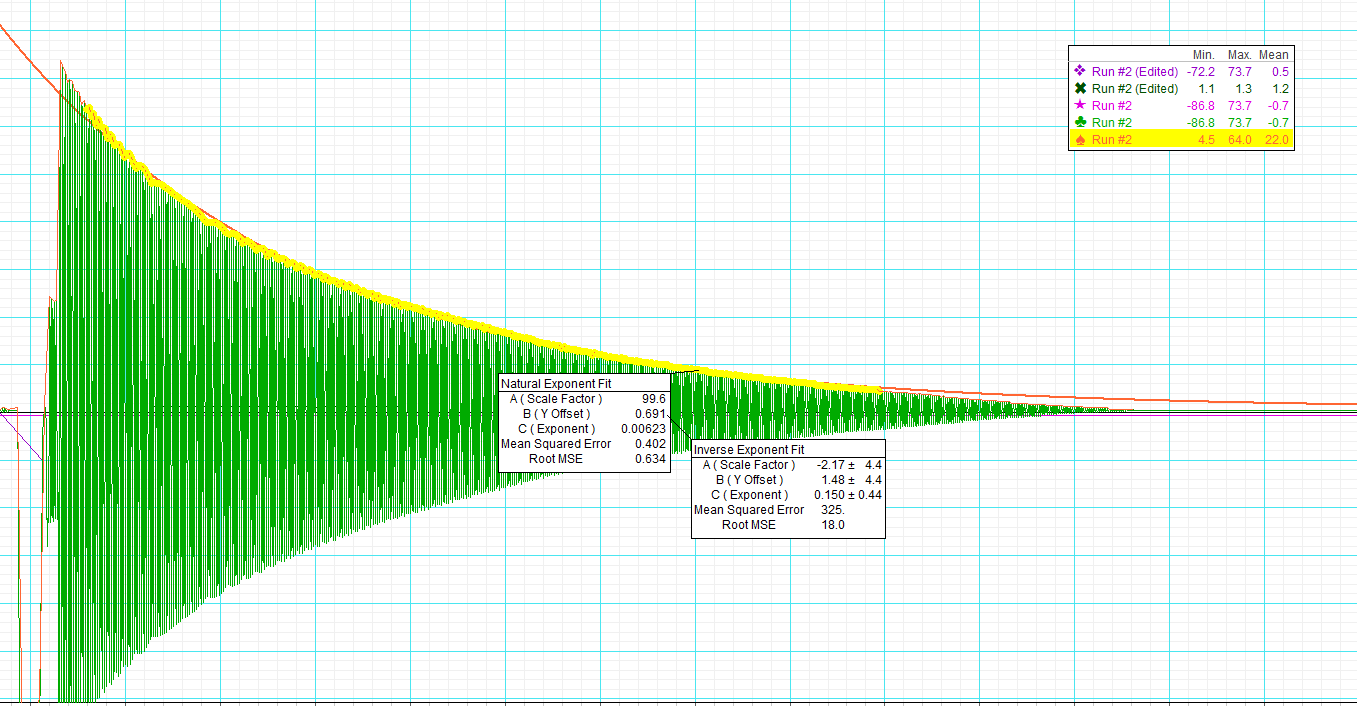
\includegraphics[width=160mm]{Capture.PNG}
\caption{Extra Credit: Calculating the Damping of a Single Pendulum $$A(t)= 97e^{-0.00594t} \therefore \gamma = 0.00594$$}
\end{figure}

\begin{figure}[ht!]
\centering
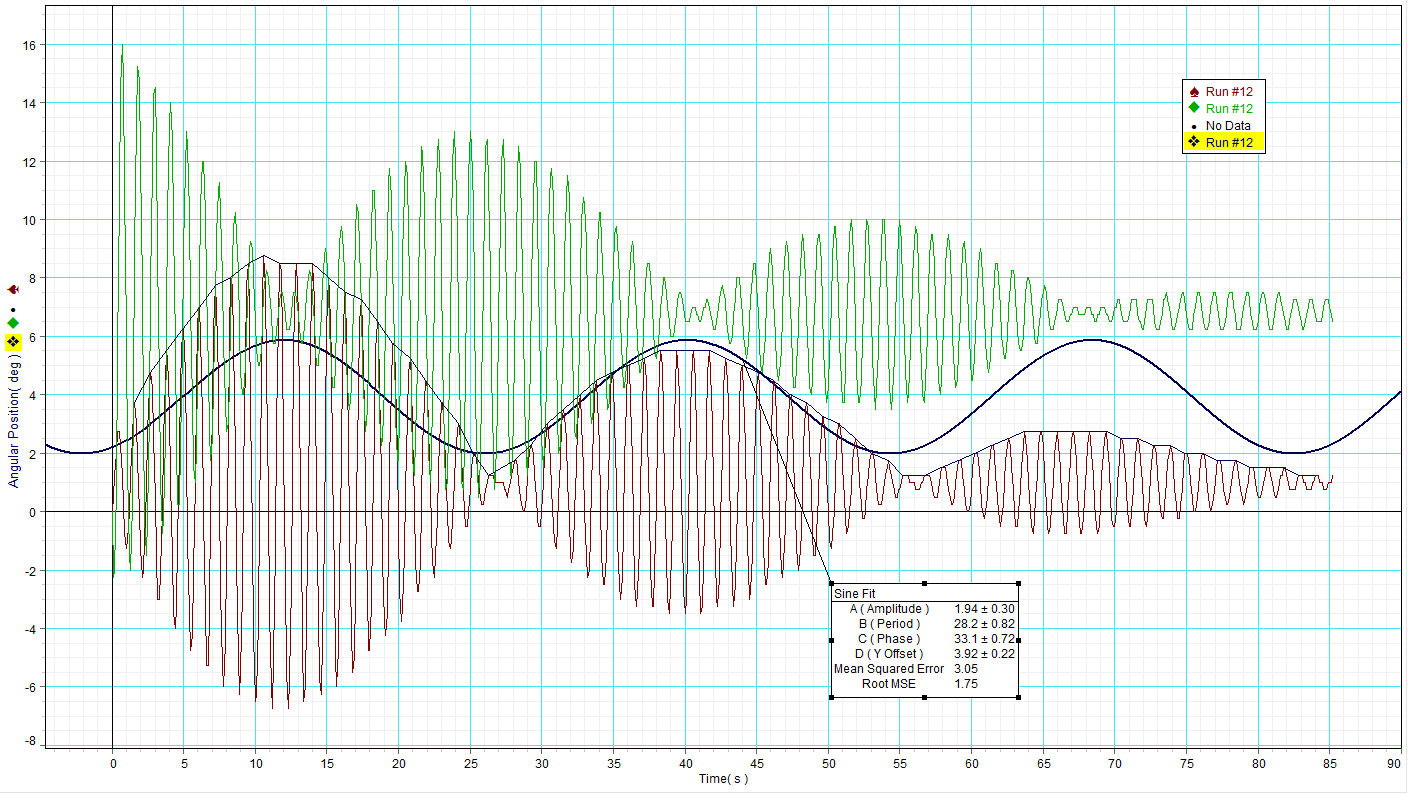
\includegraphics[width=160mm]{Capture1.PNG}
\caption{Harmonic Resonance of two Pendulums}
\end{figure}

\begin{table}[]
\centering
\caption{Experimental Data}
\label{my-label}
\begin{tabular}{llllll}
Pend Mass (g) & Rubber Band Height (cm) & $\omega_b$ & $\omega_{av}$ & $\omega_1$ & $\omega_2$ \\
74.4          & 5                       & 0.018      & 0.901         & 0.855      & 0.893      \\
74.4          & 10                      & 0.060      & 0.990         & 0.862      & 1.000      \\
74.4          & 20                      & 0.380      & 0.862         & 0.862      & 1.403     
\end{tabular}
\end{table}
\begin{table}[]
\centering
\caption{Theoretical Calculations}
\label{my-label}
\begin{tabular}{llllll}
{Pend Mass (g)} & {Rubber Band Height (cm)} & \textbf{$\omega_b$} & \textbf{$\omega_{av}$} & \textbf{$\omega_1$} & \textbf{$\omega_2$} \\
74.4                   & 5                                & 0.019               & 0.874                  & 0.855               & 0.893               \\
74.4                   & 10                               & 0.069               & 0.931                  & 0.862               & 1.000               \\
74.4                   & 20                               & 0.270               & 1.132                  & 0.862               & 1.403              
\end{tabular}
\end{table}
\pagebreak
\textbf{Questions\\}
\paragraph{Symmetric Mode:\\
\indent As we've said, the symmetric mode begins with the pendulums being displaced by the same amount in the same direction. The frequency of this normal mode is identical to the natural resonant frequency of each of the pendulums, as if the pendulums were not linked by a rubber band. In this arrangement, the rubber band between the two rods does not change it's tension, as the pendulums do not change position relative to each other. We know this from Hooke's law, which states that the tension force in a spring (or rubber band in this case) is directly proportional to the degree to which it is stretched.\\}
\paragraph{Anti-Symmetric Mode:\\ 
\indent The anti-symmetric mode is the other normal mode, and begins with the pendulums being displaced by the same amount, but in opposite directions. The frequency of this mode is much faster than that of the last, because the rubber band provides a restoring force for both of the pendulums, in addition to the force of gravity that is present in the first arrangement of the system. K, the spring constant, is equal to $\omega^2$, the frequency of the system's oscillation, divided by the ratio of the product of the pendulum's mass and length, and the vertical displcement of the rubber band from the pendulums' axes: $$\omega^2 = K\frac{l_0}{ml}$$ This value is consistent with our calculations, within an acceptable margin of error. \\}
\paragraph{Beat Frequency:\\
\indent There is a continuous "energy-tradeoff" in all systems not defined by a normal mode. The amplitude of the pendulums, and of waves in general, is proportionate to their energy. The amplitude of the pendulums at this "equal point" represents half of the energy in the system.\\}
\paragraph{Inadvertent Coupling: \\
\indent The pendulums remain coupled even when the rubber band has been removed. This is much like what Huygens initially observed in the behavior of the pendulums on his mantlepiece. The pendulums are linked by a common metal rod, which can of course transmit some vibrational energy. The beat frequency of this system is much slower than that of the previous, because it takes longer for energy to be transmitted from one pendulum to the other.\\}
\paragraph{Non-Identical Pendulums: \\
\indent When the pendulums differ in mass, we can use our general equation for motion to describe this new system, where the value of $\omega$ depends on the individual mass of each pendulum:\\} 
\medskip
\begin{equation*}
\vec{X}(t) = \left[\begin{array}{c}1 \\1\end{array}\right](a_{1}cos\omega_{1}t+ b_{1}sin\omega_{1}t) + 
\left[\begin{array}{c}1 \\-1\end{array}\right](a_{2}cos\omega_{2}t+ b_{2}sin\omega_{2}t)
\end{equation*}
\medskip
\paragraph{The pendulum with greater mass tends to have a higher amplitude than its lighter counterpart.\\ }
\paragraph{Calculating Damping Factor: \\
\indent This was our extra-credit selection. To calculate the damping factor of our two pendulum system, removed the coupling from the pendulums and set one into motion. To ensure proper rigor, we should have removed the second pendulum from the horizontal rod (see "Inadvertent Coupling"), but we figured that the damping would be great enough such that most of the pendulum's initial energy would be lost to the surrounding air molecules, rather than its stationary partner. We displaced the pendulum by a small amount, such that $sin\theta \approx \theta$, and graphed its motion over time in Data Studio. We then fit this graph of amplitude over time to an inverse exponent curve, one in which the exponent was negative. Please find the equation below figure 3. We made the assumption that our pendulum was a underdamped simple harmonic oscillator. The equation that describes this system is below, and closely resembles out best-fit line: $e^{-\gamma t} $ From this, we took gamma, our damping factor, to be 0.00594, which is remarkably low.\\}
\vspace{10mm}
\\
\paragraph{\textbf{Error Analysis:\\}Seeing as we used software and precise sensors to procure our measurements for frequency, it is unlikely that any of our experimental error came from this measurement. Instead, the small errors that we see between the experimentally- and theoretically-derived values for frequency (the frequencies of pendular motion as well as the beat frequency measured in part 3 of the experimental procedure) came from errors in other measurements, and assumptions that we made about the system as a whole. The assumption that sits least well with me is our neglecting of the pendulum rod's mass. Most of this rod is closer to the axis of rotation than the fixed mass, which gives it a smaller impact on the moment of inertia, and therefore the period, of the pendulum, but the mass of the thing is still comparable to the mass that we did measure. Taking this mass into account would decrease the frequency of oscillation considerably (see the equation on the previous page). \\}
\paragraph{By Taylor's method, the error in average frequency is given by the following equation:}
\begin{equation}
\frac {\delta \omega^2}{\omega^2} = \sqrt{ \Big(\frac{\delta K}{K}\Big) ^2 + \Big(\frac{\delta l_0}{l_0}\Big)^2 + \Big(\frac{\delta ml}{ml}\Big)^2}
\Rightarrow \delta \omega = \pm \SI{0.062}{\hertz}
\end{equation}
\paragraph{Let's compare this error for frequency to the differences between our experimentally- and theoretically- derived frequencies. Trials one and two fall comfortably within our error bars, where trial three stands slightly outside of it. This is likely due to the fact that we idealized the rubber band as a perfectly elastic string, in which force was linearly proportional to the rubber band's stretch. At a greater distance off the axis of rotation, the rubber band stretches more, and force no longer scales directly with displacement. In order to rectify this error, we would have to create some function $F(x)$ for the spring, polynomial or otherwise, instead of simplifying with some constant $K$. \\}
\vspace{10mm}
\paragraph{\textbf{Conclusions:\\}
All in all, this was the most successful experiment I've conducted here at NYU. My partner and I were able to use Data Studio to our advantage, which was a rare treat. We used the software to compute best-fit sine curves for each state of the coupled pendulum system. We even able to compute a value for the damping factor of our system by graphing the oscillation of a single pendulum over a significant time-frame, and fitting this graph to and inverse-exponent curve. We were surprised by how little power was lost to non-conservative forces! We stupidly chopped-off the time scale in this graph, but the pendulum was in motion for a duration of over four minutes.}
\paragraph{\LaTeX, yo} 
\vfill
\end{document} 





